\section{Liyana Majdah Rahma(1174039)}
\subsection{Pengertian}

\subsection{Sejarah}
\subsection{Koordinat}
\subsection{Data Geospasial}
Data dalam Sistem Informasi Geografis terdiri dari dua komponen yaitu data spasial dan data attribute. Kata Geospasial terdiri dari dua katayaitu geo dengan spasial, Geo sendiri memiliki arti bumi sedangkan spasial memiliki arti ruang. Jika di gabungkan geospasial merupakan data bereferensi geografis atas resprentasi obyek dibumi. Selain itu juga geospasial  di bagi lagi menjadi dua bagian,yaitu data garis dengan data geometri. Data tersebut terdiri dari tiga elemen berupa,garis,titik,dan luasan. Serta Data geospasial berbentuk raster dan vector.

Model data vector merupakan data yang menampilkan,menempatkan,dan menyimpan data spasial dengan menggunaka titik dan garis,bahkan selain itu juga dapat berupa bentuk polygon. Biasanya jenis tipe data ini terdapat pada peta. Dalam format vector , bumi di representasikan sebagai suatu mosaic dari sebuah garis,polygon (dimana daerah yang dibatasi oleh garis yang berawal dan berakhir pada titik yang sama. Setiap Data pada vector dapat mempunyai informasi-informasi yang berasosiasi satu dengan yang lainnya misalnya penggunaan pada sebuah label untuk menggambarkan informasi pada suatu lokasi. Ada pun Keuntungan utama dari format data vektor yaitu adalah ketepatan dalam merepresentasikan fitur titik, batasan dan garis lurus. Hal tersebut juga  sangat berguna untuk analisa yang membutuhkan ketepatan posisi, misalnya pada basisdata batas-batas kadaster. Selain itu juga terdapat Kelemahan  saat menggunakan data vektor yang utama adalah ketidakmampuannya dalam mengakomodasi perubahan gradual.


Selanjutnya yang kedua model data raster merupakan data yang dihasilkan dari sistem Penginderaan Jauh. Pada data raster juga, obyek geografis direpresentasikan sebagai struktur sel grid yang disebut dengan pixel (picture element).  Selain itu  data raster, memiliki  resolusi (definisi visual) tergantung ukuran pixel-nya.  Resolusi  pixel juga dapat  menggambarkan ukuran sebenarnya di permukaan bumi yang diwakili oleh setiap pixel pada citra. Jika Semakin kecil ukuran permukaan bumi yang direpresentasikan oleh satu sel, maka semakin tinggi  hasil resolusinya. Begitupun data raster sangat baik untuk direpresentasikan pada batas-batas yang berubah secara gradual, misalnya pada  jenis tanah, kelembaban tanah, vegetasi, suhu tanah, dan lain-lainnya.


\subsection{Link}
\href{https://youtu.be/hFj3s-4dte8}{kli ini bro}
\subsection{Plagiarism}
\begin{figure}[H]
	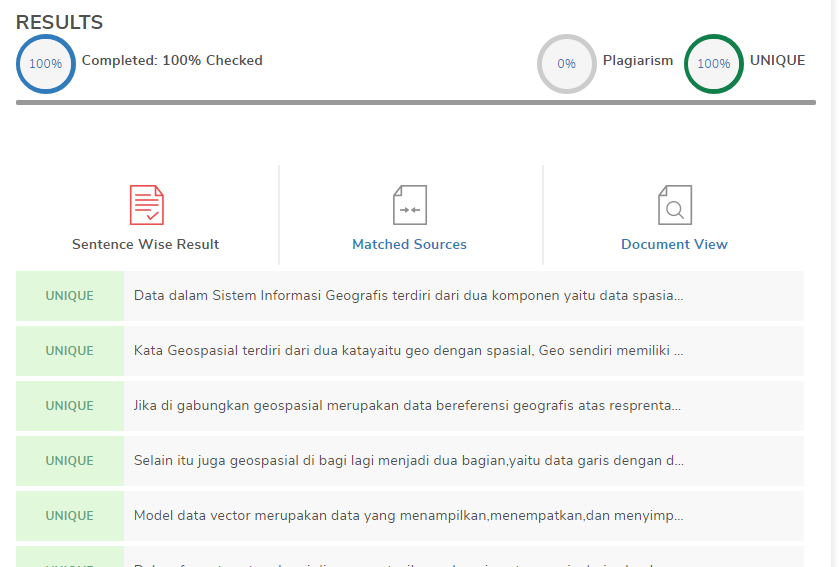
\includegraphics[width=4cm]{figures/1174039/plagiat.png}
	\centering
	\caption{Plagiat.}
\end{figure}

